\documentclass[11pt]{paper}

\usepackage{amsmath}
\usepackage{geometry}
\usepackage{chemarrow}
\usepackage{amssymb}
\usepackage{palatino}
\usepackage{mwe}
\usepackage{listings}
\usepackage{graphicx}
\usepackage{geometry}
\usepackage{setspace}
\usepackage{extarrows}
\usepackage{tikz}
\usepackage{float}


\onehalfspacing
%margin
\geometry{papersize={8.5in,11in}}
\geometry{left=1in,right=1in,top=1in,bottom=1in}
\pagestyle{plain}

%title
\author{\textbf{Team P}\\\large Yixuan Li (yl3757), Jenny Liu (jl3957),  Shrey Goel (sg3502), Muktesh R. Waghmare (mw3199)}

\title{Deep Portfolio Management\\\large Semester Project for IEOR 4720 Deep Learning}
\usepackage{indentfirst}
\setlength{\parindent}{2em}



\begin{document}

	%generate the title
	\maketitle
	%\tableofcontents
	%\newpage

	\abstract{Financial portfolio management is the process of constant redistribution of a fund into different financial products. Deriving inspiration from Zhengyao Jiang, Dixing Xu and Jinjun Liang on providing a deep machine learning solution to the portfolio management problem, we tried replicating the results of the paper and make further improvements. The paper describes a framework consisting of the Ensemble of Identical Independent Evaluators (EIIE) topology, a Portfolio-Vector Memory (PVM), an Online Stochastic Batch Learning (OSBL) scheme, and a fully exploiting and explicit reward function realized in a Convolutional Neural Network (CNN). Operating in a cryptocurrency environment, we ran back-test experiments with a trading period of 30 minutes on 5 minute tick data. Post successful replication of the results described in the paper, we focused our attention on examining the characteristics of the model and making enhancements to the model such as finding better initialization and activation function, adding slippage to more accurately represent bactesting returns and accessibility for more input data types to make the model more versatile.}
	\keywords{Machine learning; Convolutional Neural Networks; Deep Learning; Cryptocurrency; Bitcoin; Algorithmic Trading; Portfolio Management; Quantitative Finance }


	\section{Problem Overview}
		In this project, we are studying a portfolio management problem where we try to maximize the value of a actively traded bitcoin portfolio by constantly rebalancing using weight vector generated from a CNN neural network. In this work, trading algorithms are time-driven, the total trading time of roughly two month is divided into periods of equal lengths T=30 min. At the beginning of each period, the trading agent reallocates the fund among the assets. 

		For data sourse, we used public available 5min Bitcoin tick data automatically downloaded using web-scrapping from the Poloniex website. In each trading period of 30 minutes, we used "open","high","close" from certain historical periods as three features to feed in the neural network. Former weight vector is also feeded in the network as input. Then, Ensemble of Identical Independent CNN Evaluators topology is adopted as shown in the following figure. Each assets is evaluated in a seperate Neural Network before being assigned a weight using softmax function.

		The whole process included training the trading policy in random mini-batches, select models using a validation period with the same length of testing period by comparing portfolio value, max drawdown and Sharpe Ratio. Finally we apply the best trading policy to the testing period. 


	

	


	\section{Model Replication}
		\subsection{Tuning The Parameters}
		The github code for this paper is streamlined, therefore we first try to set up the project, re-run the code and tune the hyperparameters with hope to replicate the results stated in the paper. Since CNN structure has the best results, we focus on CNN and use this as a benchmark for further study.

		Table 1 and Figure 2 shows the portfolio performance with different hyperparameters and the number shows the order of our attempts. Here for illustration purpose, we only show the result of time period from 2016-09-07 to 2016-10-28. Starting from the pre-determined parameter in github, we gradually adjust the hyperparameters to achieve better results. Each train-validation process takes about 8 hours and the time gets longer with higher training steps. Although it is time consuming, by increasing training steps, we can improve the performance in an obvious way (comparing agent No.7 and No.10). 



		\subsection{Comparing Results With The Paper}
		The paper shows the testing result in three different time period and we would like to relicate the process by using exact same period with out best tuned parameter. 
		\begin{table}[h]
\begin{tabular}{|c|c|c|c|c|c|c|c|c|c|}
\hline
            & \multicolumn{3}{c|}{2016-09-07 to 2016-10-28} & \multicolumn{3}{c|}{2016-12-08 to 2017-01-28} & \multicolumn{3}{c|}{2017-03-07 to 2017-04-27} \\ \hline
            & MDD    & PV        & SR    & MDD     & PV       & SR    & MDD    & PV        & SR    \\ \hline
Paper       & 0.224           & 26.695    & 0.087           & 0.216            & 8.026    & 0.059           & 0.406           & 31.747    & 0.076           \\ \hline
Replication & 0.143           & 8.556     & 0.077           & 0.226            & 2.994    & 0.0449          & 0.398           & 88.415    & 0.101           \\ \hline
\end{tabular}
\caption{Comparison of results summary of paper and our replication}
\end{table}
\footnote[1]{MDD: Max Drawdown, PV: final portfolio value, SR: Sharpe Ratio}
	
	From Table 2 we can see that there is still discrepency between our results and the paper's. We think that this is due to the randomness in the mini-batch training process. However, we manage to keep the orders of the PV for three different period with the third period highest and second period lowest.



	


	\section{Modification and Improvements}
		\subsection{Alternative Data Source}
		The paper provides code to download cryptocurrency data from Poloniex to be used for training and testing, limiting the scope of the data to only cryptocurrencies with the highest volumes.

		We added the functionality of writing our own database using SQLite3. The data would come from csv files that the user provides. This adds a lot more flexibility to what kind of data can be used with the neural networks. The rest of the program functions as usual.

		Users can upload their own csv file and the csv file would then be turned into a pandas dataframe, which will then be converted to a SQLite3 database that integrates with the rest of the code as long as the format of the csv is as follows:\\

		\begin{tabular}{|l|l|l|l|l|l|l|l|l|}
		\hline
		date       & coin & high & low & open & close & volume & quoteVolume & weightedAverage \\ \hline
		yyyy/MM/dd & name & -    & -   & -    & -     & -      & -           & -               \\ \hline
		\end{tabular}


		\subsection{Market Impact and Trading Slippage}
		The paper made an assumption of zero slippage in the market. However, given the rebalancing period of 30 minutes, it is reasonable to consider market impact. Therefore, to improve the model, we added linear market impact to the quoted price.

		At each rebalancing time, suppose we have a position of $x_i$, we assume the price will increase from $p_t$ to $p_t+\alpha x_i$, where $\alpha$ is the degree of market impact. This impact will increase the cost of future purchase and decrease the cost of future sale.

		The transaction remainder factor $0<\mu_t<1$ provides a way to calculate the shrink of portfolio value from $p_t$ to $\mu_t p_t$ . We added the market impact α to the model and get the following equation:
		\[(1-c_p-\alpha) [w'_{t,0}+(1-c_s+\alpha)\sum_{i=1}^m(w_{t,i}'-\mu_tw_{t,i})^+-\mu_tw_{t,0}]=\sum_{i=1}^m(\mu_tw_{t,i}-w'_{t,i})^+\] where $w_t'$ and $w_t$is the portfolio weight before and after rebalancing at time t.

		Using the fact that $w'_{t,0}+\sum_{i=1}^m(w_{t,i}'=1=w_{t,0}+\sum_{i=1}^m(w_{t,i}$, the equation is simplified to 
		\[\mu_t=\frac{1}{1-(c_p+\alpha)w_{t,0}}[1-(c_p+\alpha)w'_{t,0}-(c_s+c_p-(c_s-\alpha)(c_p+\alpha))\sum_{i=1}^{m}(w'_{t,i}-\mu_tw_{t,i})^+]
		\]
		$\mu_t$ doesn't have an explicite solution so we use Newton's Method to solve for $\mu_t$ recursively.
		
		\subsection{Structure of Neural Network}
		To further improve the structure of neural network, we evaluated the performance/convergence speed of the loss function using different initialization schemes, activation functions. 
		
		Tools such as Tensorboard summary operations were used for collecting the data. The code is streamlined so that we can easily gauge the convergence performance. For instance, we can attach the tf.summary.scalar to the variable that held the loss function value.  Likewise, it also allows us to visualize the distribution of gradients and weights. This was done by attaching the tf.summary.histogram operator to the gradient outputs and the variables storing the weights. 

		\subsubsection{Weight Initialization}
		The paper suggests using truncated normal initialization. Using tensorboard, we visualized the loss curve for this configuration and observed a plateau in the beginning. Plateau at the beginning shows initialization sensitivity during which period the network doesn’t learn much in the initial steps.


		Addressing this initialization sensitivity, we used Xavier initialization with sampling from uniform distribution and with standard deviation scaled by a factor of $\sqrt{\frac{1}{\# \ of\ inputs}} $. we see that the plateau region has decreased, and the network trains nicely.


		Deriving inspiration from the paper Delving Deep into Rectifiers: Surpassing Human-Level Performance on ImageNet Classification by Kaiming He, Xiangyu Zhang, Shaoqing Ren and Jian Sun from Microsoft Research which suggests using scaled variance for networks with ReLU activation units, we tried initializing our network by sampling from random normal distribution with standard deviation scaled  by a factor of $\sqrt{\frac{2}{\# \ of\ inputs}} $. A plot of loss with respect to iterations is as follows. As evident from the graph, the loss did not necessarily decrease with the epochs and hence, we decided to use Xavier initialization. This phenomenon is generally observed when learning rate is high, which might also explain faster learning at the beginning of the curve below.




		\subsubsection{Activation Function}
		The paper suggests using ReLU activation function and delivers exceptional results. We were able to replicate the results as written in the paper. However, when we used PReLU activation function to train neural networks, we could see a significant improvement in the portfolio performance. The information and Sharpe ratios have improved significantly with an improvement in the drawdown. 

	
		Moreover, we can train the network in 1.4 million epochs as compared to 2 million epochs with the ReLU activation earlier. The loss function curve below shows smooth training of the network with PReLU activation with no initialization sensitivity. This can be attributed to the fact that a lot of neurons might remain dead in ReLU and the gradient doesn’t flow through the network.





	\section{Conclusion and Further Improvements}
	\subsection{Project Review}
	In this project, we first try to replicate the paper with an CNN EIIE structure after a time-consuming process of tuning the parameters. We noticed the similarity in performance orders of three testing period as well as the discrepency in portfolio values. Since randomness exists in the traiing process, it is difficult to get the same parameters as the authors.

	After the replication process, we endeavored to seek improvements for the model in adding function for alternative data source, adjusting for market impact and modifying the structure of neural networks. We believe these improvements added the robustness and enhanced performance for this portfolio management strategy.

	Overall, it is a great learning experience and our team members get a more hand-on understanding of deep learning knowledge learnt in class, portfolio management problem and cryptocurrency market. Our team members are also grateful for this memorable teamwork experience. Almost everyone is dedicated and engaged.\footnote[1]{Shrey, Jenny and Yixuan contributes great time and efforts to in replicating the paper (section 2) and making improvements (section 3) over the semester. This report is composed by Yixuan with great ideas and contributions from Shrey and Jenny. However, it is regrettable that Muktesh didn't have much chance to participate in this project due to some personal reasons. The project could surely be better with Muktesh's contribution.} We have arranged many group meetings to discuss possible plans and spent much time afterwards learning the code and making modifications. It is the collaborative efforts that generate the final version of our project.
	
	\subsection{Further Improvements}
	The result of our replication in section 2 (Table 2) motivated us to think about the validity and robustness of this portfolio management strategy in under various market conditions. We can see the portfolio value can vary from 2.994 to 88.415 after just three month. It is possible that our portfolio strategy is most useful under certain market conditions that is suited for this strategy. In the future, one improvement can be to study the robustness of the trading strategy.

	Also, by adding the function to write our own database, we hope to encourage people to apply this strategy to other asset classes such as foreign exchange or commodity for a wider use. Cryptocurrency market is pretty unique compared to other traditional assets and it is meaningful to see whether the strategy still works without this market uniqueness.

	\section*{Reference}
	1. Jiang Z, Xu D, Liang J. A deep reinforcement learning framework for the financial portfolio management problem[J]. arXiv preprint arXiv:1706.10059, 2017.

	2. He K, Zhang X, Ren S, et al. Delving deep into rectifiers: Surpassing human-level performance on imagenet classification[C]//Proceedings of the IEEE international conference on computer vision. 2015: 1026-1034.

	3. Agarwal A, Hazan E, Kale S, et al. Algorithms for portfolio management based on the newton method[C]//Proceedings of the 23rd international conference on Machine learning. ACM, 2006: 9-16.
	\section*{Note}
	Github Repo: https://github.com/ShreyGoel/DeepLearningForked\\

	

	Contributors:

	Shrey Goel: ShreyGoel

	Jenny Liu: jjenster

	Yixuan Li: Candice-lyx


	\newpage
	\section*{Appendix}
	\subsection* {A. Model Structure}
			\begin{figure}[h]
			\centering  
			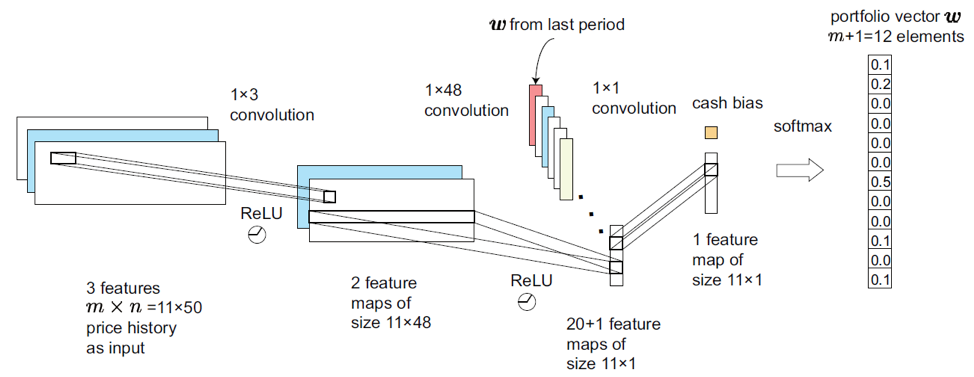
\includegraphics[width=0.7\linewidth]{cnn.png} 
			\caption{CNN EIIE Architecture} 
			\label{fig:cnn}   
		\end{figure}
	\subsection*{B. Tuning the Hyperparameters}
			\begin{figure}[h]%%图
			\centering  
			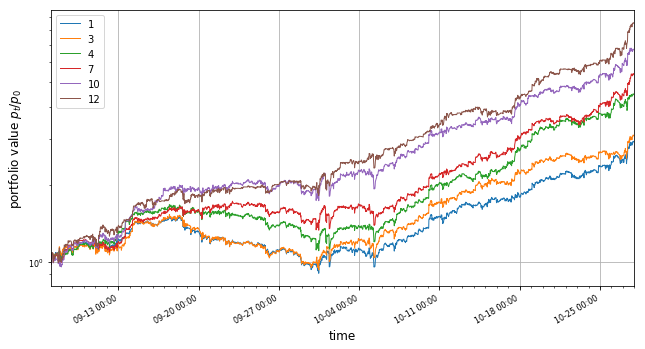
\includegraphics[width=1\linewidth]{tune.png} 
			\caption{Portfolio Performance with different hyperparameters} 

		\end{figure}
		\begin{table}[]

		\setlength{\tabcolsep}{1mm}{
\begin{tabular}{|p{3cm}|p{4.5cm}|l|l|l|l|l|l|l|l|}
\hline
                           &                                                                                        & \multicolumn{6}{c|}{Trading Agent Number}                                 \\ \hline
Hyperparameters            & Description                                                                            & 1        & 3        & 4        & 7        & 10       & 12       \\ \hline
batch size                 & Size of mini-batch during training                                                     & 100      & 100      & 50       & 50       & 50       & 50       \\ \hline
window size                & Number of trading periods in input price matrix                                        & 50       & 50       & 50       & 50       & 50       & 50       \\ \hline
trading period (second)    & Time interval between portfolio rebalance                                              & 1800     & 1800     & 1800     & 1800     & 1800     & 1800     \\ \hline
total steps                & number of steps for training                                                           & 8000     & 30000    & 30000    & 30000    & 2.00E06  & 2.00E06  \\ \hline
regularization coefficient & L2 regularization coefficient                                                          & 5.00E-08 & 5.00E-08 & 5.00E-08 & 1.00E-08 & 1.00E-08 & 1.00E-08 \\ \hline
learning rate              & Parameter of Adam optimization                                                         & 0.00028  & 0.00028  & 0.00028  & 0.00028  & 0.00028  & 3.00E-05 \\ \hline
rolling steps              & Number of online training steps for each period during cross-validation and back-tests & 85       & 85       & 85       & 30       & 30       & 30       \\ \hline
\end{tabular}
}
		\caption{Hyperparameters for different trading agents }
\end{table}
	\subsection*{C. Weight Initialization}
			\begin{figure}[h]
			\centering  
			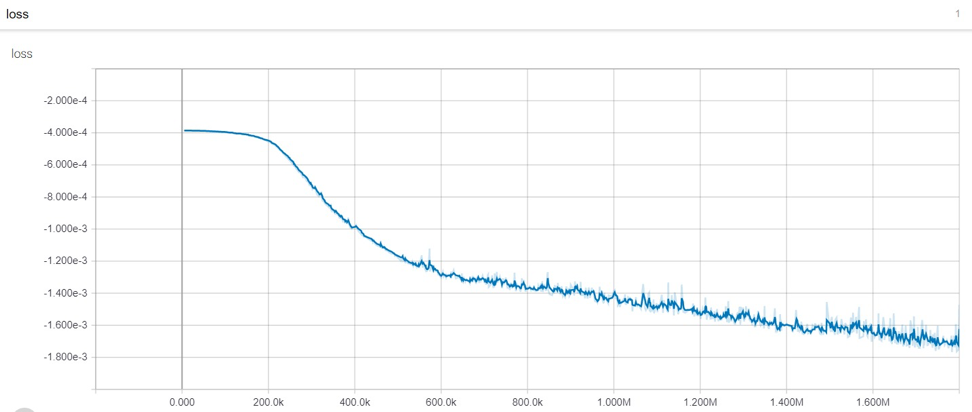
\includegraphics[width=0.7\linewidth]{initialization1.png} 
			\caption{Loss curve for truncated normal initialization}   
		\end{figure}
			\begin{figure}[H]%%图
			\centering  
			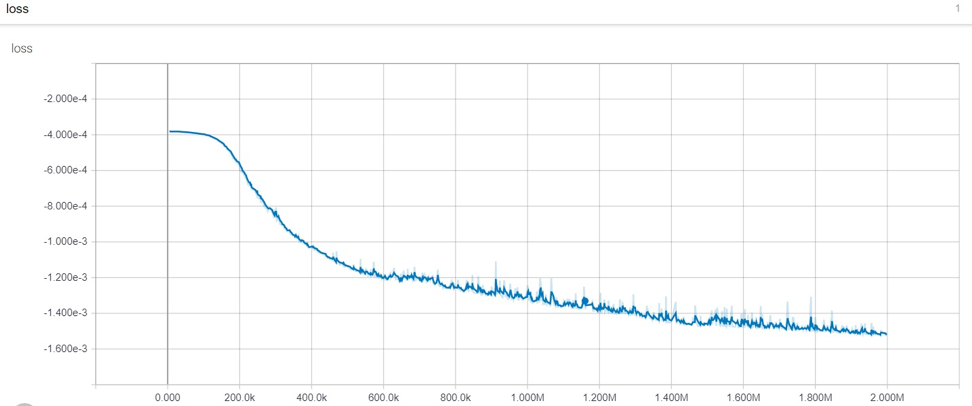
\includegraphics[width=0.7\linewidth]{initialization2.png} 
			\caption{Loss curve for Xavier initialization} 
		\end{figure}
			\begin{figure}[H]
			\centering  
			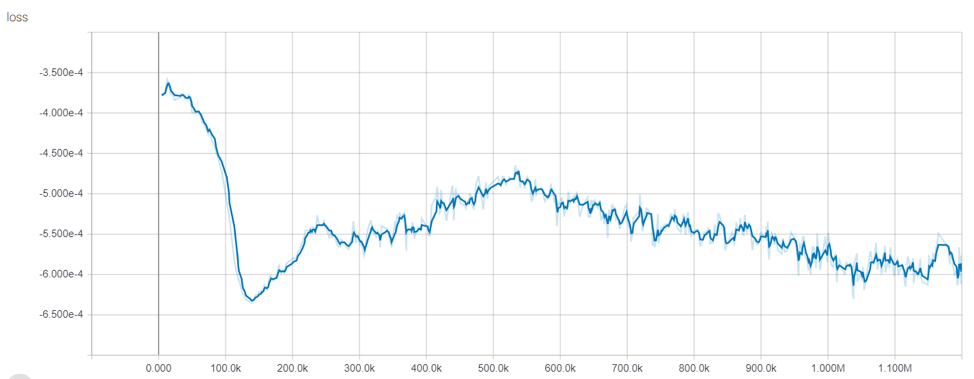
\includegraphics[width=0.7\linewidth]{initialization3.png} 
			\caption{Loss curve for scaled-variance initialization} 
		\end{figure}
	\subsection*{D. Activation Function}
			\begin{figure}[H]
			\centering  
			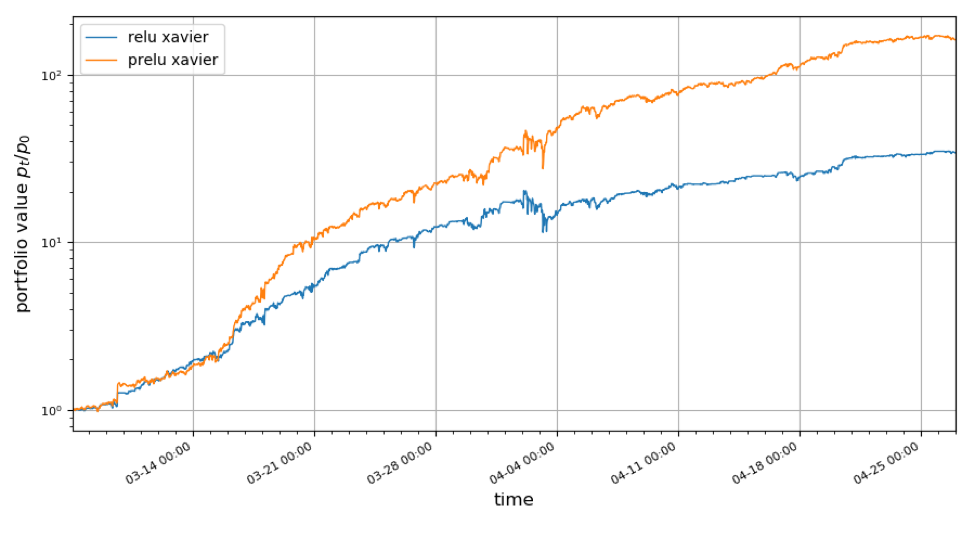
\includegraphics[width=0.7\linewidth]{activation.png} 
			\caption{Portfolio Performance with different activation functions} 
		\end{figure}
		\begin{figure}[H]%%图
			\centering  
			
\includegraphics[width=1\linewidth]{activation2.png} 
			\caption{Portfolio Performance with different activation functions} 
		\end{figure}
			\begin{figure}[H]
			\centering 
			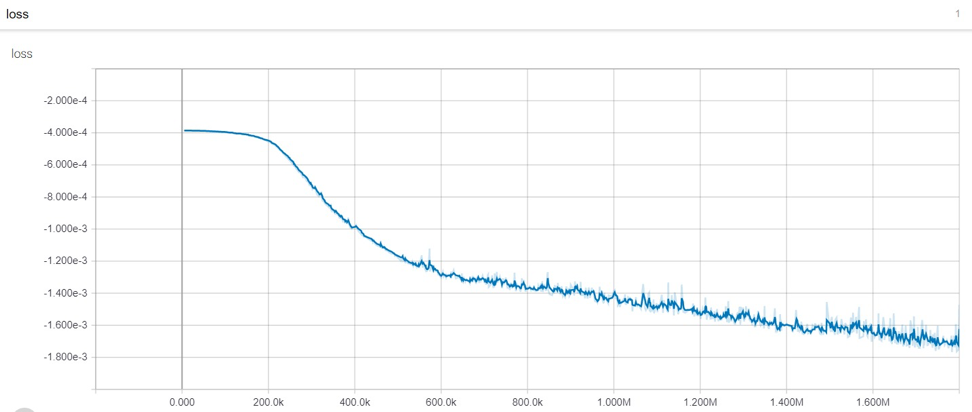
\includegraphics[width=0.7\linewidth]{initialization1.png} 
			\caption{Convergence speed of ReLU}
			\label{fig:cnn} 
		\end{figure}
		\begin{figure}[H]
			\centering  
			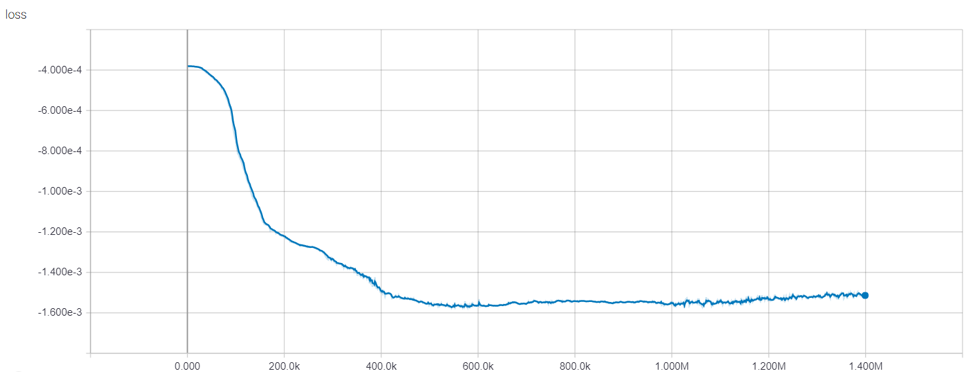
\includegraphics[width=0.7\linewidth]{prelu.png} 
			\caption{Convergence speed of PReLU} 
			\label{fig:cnn} 
		\end{figure}



	
	





	











		%\subsection*{3)}

\end{document}